\label{chap:turbu_categories}
\newthought{The}~horizontal scales of planetary geostrophic turbulence are usually so much
larger than the vertical, that due to the gyroscopic rigidity of fluid motion
in a rotating frame of reference, the turbulence is practically invariant in
the vertical. Two-dimensional motion has the odd, counter-intuitive quality of
cascading towards \textbf{larger} instead of \textbf{smaller} scales, as would be
expected from 3-dimensional flow. This appendix is an attempt to explain
this peculiar phenomenon heuristically.
%%%--------------------------------------------------------------------
\begin{subequations} \label{eq:EQS1}
\begin{align}
	\frac{D \vec{u}}{D t}
	+
	\vec{\Omega} \times \vec{u}
	&=
	- \frac{1}{\rho} \vec{\nabla} p
	+
	\nu  \vec{\nabla}^{2} \vec{u}
	+
	 \vec{g}
	  \label{eq:NS2} \\
	%%####################################################################
	%%####################################################################
	\frac{D m}{D t}
	&=
	0 \label{eq:konti1}\\
	%%####################################################################
	%%####################################################################
	\frac{D \vec{\omega_{a}}}{D t}
	&=
	\left( \vec{\vec{\omega}_{a}} \cdot \grad \right) \vec{\vec{u}}
	+
	\B
	+
	\nu \grad^2 \vec{\omega}
		\label{eq:vort1}\\
	%%####################################################################
	%%####################################################################
	\frac{D \Ek}{D t}
	&=
	-
	\vec{u}_{h} \cdot \frac{1}{\rho} \grad_{h} p
	+
	\nu \left(
	\frac{1}{2}\grad^2 \vec{u}^2 - \norm{\grad \vec{u}}^2
\right)
	\label{eq:Ekin1}\\
	%%####################################################################
	%%####################################################################
	\frac{D \Em}{D t}
	&=
	\nu	\left(
	\frac{1}{2}\grad^2 \vec{u}^2 - \norm{\grad \vec{u}}^2
	\right)
	\label{eq:Emech1}\\
	%%####################################################################
	%%####################################################################
	\frac{D \enstro}{D t}
	&=
	\vec{\omega}\cdot \left( \vec{\vec{\omega}_{a}} \cdot \grad \right) \vec{\vec{u}}
	+
	\vec{\omega}\cdot  \nu \grad^{2} \vec{\omega}
	\label{eq:enst1}
\end{align}
\end{subequations}

%%%--------------------------------------------------------------------

\newthought{Consider}~the equations of motion on a rotating spherical planet with all body forces
combined in $\vec{g}$, which shall always be perpendicular to
the surface of a Newtonian fluid at rest. Applying the curl to \eqref{eq:NS2}
also yields a vorticity equation\derref{der:vort}.
Scalar multiplication with $\vec{u}$ reveals a prognostic, kinetic-energy-per-unit-mass budget\derref{der:Ek}.
Analogously, scalar multiplication of \eqref{eq:vort2} with $\vec{\omega}_{a}$ yields an equation
for the macroscopic enstrophy density per unit mass\derref{der:enstro}. Finally, adding a term for potential energy to \eqref{eq:Ekin1} yields an equation for mechanical energy\derref{der:Em}.

\begin{figure}
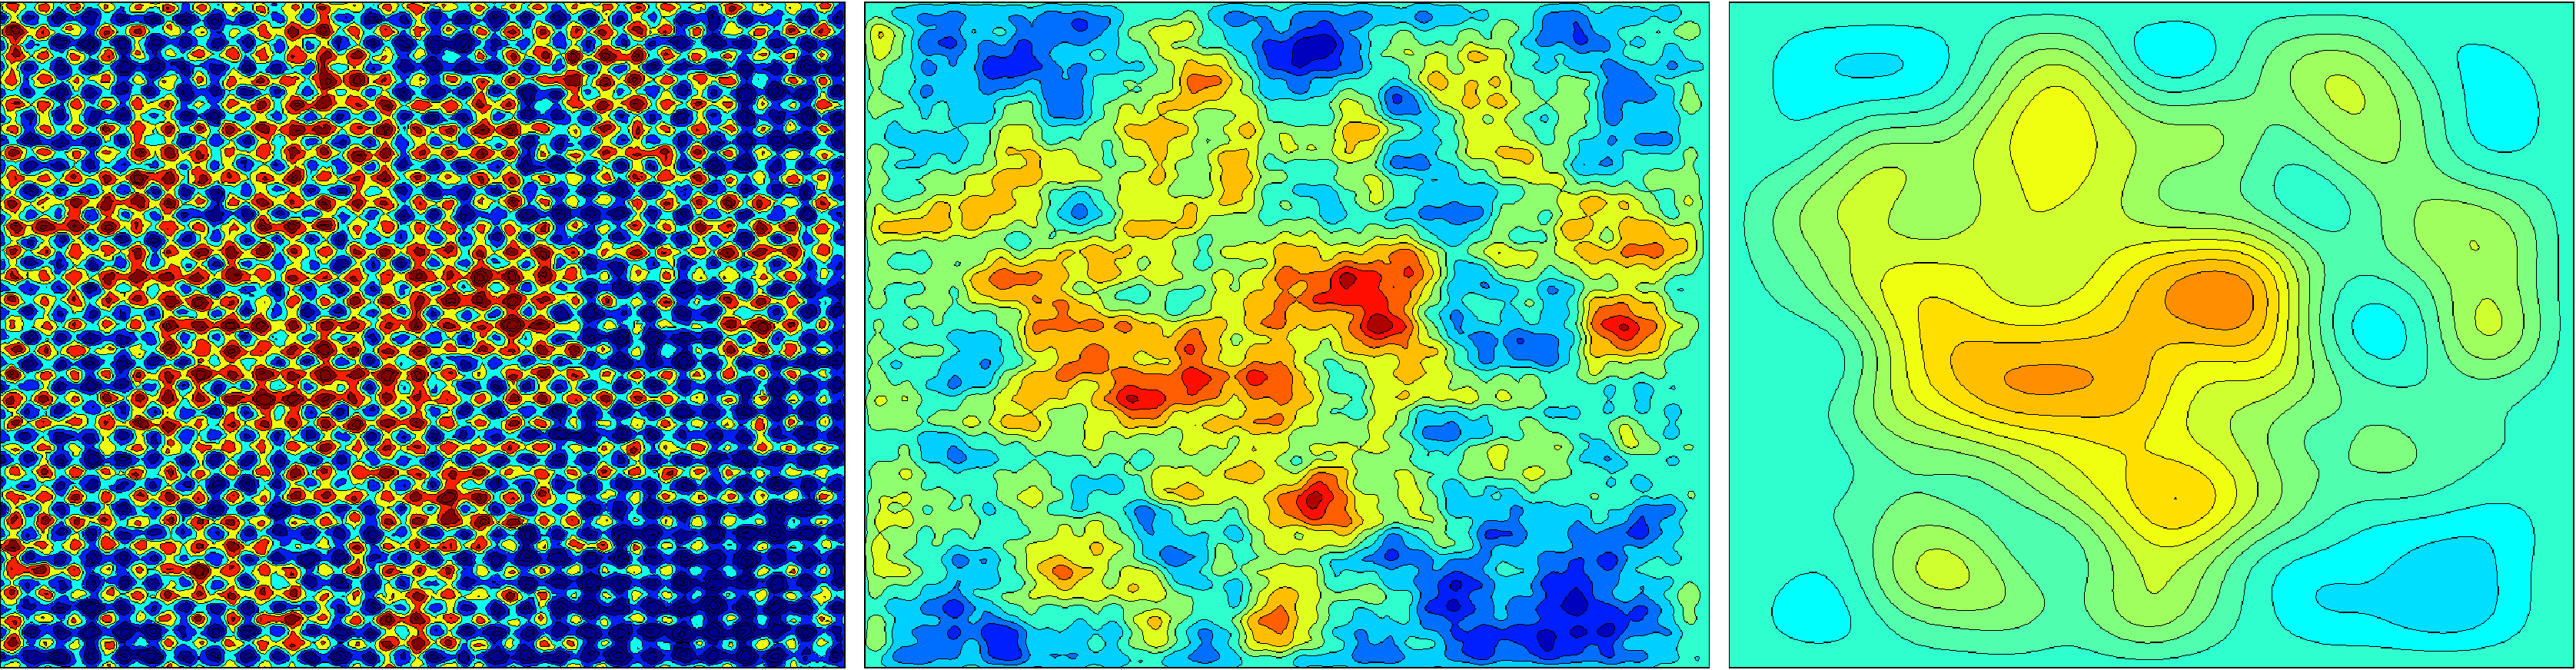
\includegraphics[width=\textwidth]{PSI.pdf}
\caption{1) 2D turbulence with several sinusoidal and random signals as initial condition, 2) at a later time 3) at a much later time. Code from
\citet{Seibold2008a}.}
\label{fig:PSI}
\end{figure}


%%%####################################################################
%%%####################################################################
\begin{fullwidth}
\begin{turbu}[Non-rotating Tank]\label{turb:tank}

\newthought{Consider}~first a 3 dimensional non-rotating volume of fluid of constant density with horizontal and vertical dimensions of equal scale.
 \Eqsref{eq:EQS1} then reduce to (ignoring $\Ek$):
%%--------------------------------------------------------------------
\begin{subequations}
\begin{align}
	\frac{D \vec{u}}{D t}
	&=
	- \frac{1}{\rho} \grad p
	+
	\nu  \vec{\nabla}^{2} \vec{u}
	+
	 \vec{g}
	 \\
	%%####################################################################
	%%####################################################################
	\div \vec{u}
	&=
	0
	\label{eq:konti2}\\
	%%####################################################################
	%%####################################################################
	\frac{D \vec{\omega}}{D t}
	&=
	\left( \vec{\vec{\omega}} \cdot \grad \right) \vec{\vec{u}}
	+
	\nu \grad^2 \vec{\omega}
	\label{eq:vort2}\\
	%%####################################################################
	%%####################################################################
	 \addtocounter{equation}{+1}
	%%####################################################################
	%%####################################################################
	\frac{D \Em}{D t}
	&=
	\nu\left(
	\frac{1}{2}\grad^2 \vec{u}^2 - \norm{\grad \vec{u}}^2
	\right)
	\label{eq:Emech2}\\
	%%####################################################################
	%%####################################################################
	\frac{D \enstro}{D t}
	&=
	\vec{\omega}\cdot \left( \vec{\vec{\omega} } \cdot \grad \right) \vec{\vec{u}}
	+
	\vec{\omega} \cdot  \nu \grad^{2} \vec{\omega}
	\label{eq:enst2}
\end{align}
\end{subequations}

%%--------------------------------------------------------------------

\newthought{If}~we further assume the viscosity $\nu$ of the fluid to be infinitely small, \eqref{eq:Emech2} and \eqref{eq:enst2} reduce to
%%--------------------------------------------------------------------
\begin{subequations}
\begin{align}
	%\frac{D \vec{u}}{D t}
	%&=
	%- g \grad h
	%+
	%\nu  \vec{\nabla}^{2} \vec{u}
	%+
	 %\vec{g}
	 %\\\
	 \addtocounter{equation}{+1}
	%%%####################################################################
	%%%####################################################################
	%\div \vec{u}
	%&=
	%0
	%\label{eq:konti3}\\
	 \addtocounter{equation}{+1}
	%%%####################################################################
	%%%####################################################################
	%\frac{D \vec{\omega_{a}}}{D t}
	%&=
	%\left( \vec{\vec{\omega}} \cdot \grad \right) \vec{\vec{u}}
	%+
	%\nu \grad^2 \vec{\omega}
	%\label{eq:vort2}\\
	 \addtocounter{equation}{+1}
	%%####################################################################
	 \addtocounter{equation}{+1}
	%%####################################################################
	\frac{D \Em}{D t}
	&=
	0
	\label{eq:Emech3}\\
	%%####################################################################
	%%####################################################################
	\frac{D \enstro}{D t}
	&=
	\vec{\omega}\cdot \left( \vec{\vec{\omega}} \cdot \grad \right) \vec{\vec{u}}
	\label{eq:enst3}
\end{align}
\end{subequations}

%%--------------------------------------------------------------------

\newthought{In}~the absence of friction the mechanical Energy of the parcel of fluid is conserved.
In contrast, neither enstrophy nor vorticity itself are conserved.
%Not even when initial conditions of zero relative vorticity are assumed.
%Think of, for example the case where $\Omega$ scales much larger than $\omega$ e.g. slow, large-scale circulation.
Velocity gradients will tilt and stretch the parcel resulting in
changes in relative vorticity so as to conserve the parcel's total
angular momentum. There is no preference for dimension. The motion is
simply turbulent akin to air blowing through a room.
\end{turbu}

%%%####################################################################
%%%####################################################################
\begin{turbu}[Rotating Tank]\label{turb:rottank}
Next consider the tank from \cref{turb:tank} to be rotating at some
high constant frequency $\vec{\Omega/2}\cdot\unitvec{z}$, so that all terms void of
$\vec{\Omega}$ are small versus those containing $\vec{\Omega}$ while all
derivatives of $\vec{\Omega}$ vanish for its constancy. Again, imagine some
magical mix of body forces, so that $\vec{g}\cdot\unitvec{z}=-g$.
%%--------------------------------------------------------------------
\begin{subequations}
\begin{align}
	 \frac{D \vec{u}_{h}}{D t}
	&=
	-
	\vec{\Omega} \times \vec{u}_{h}
	+ g \grad \eta
	%+
	%\nu  \vec{\nabla}^{2} \vec{u}
	 \label{eq:NS4} \\
	%%####################################################################
	%%####################################################################
	%\div \vec{u}
	%&=
	%0
	%\label{eq:konti1}\\
	 \addtocounter{equation}{+1}
	%%####################################################################
	%%####################################################################
	\frac{D \vec{\omega}}{D t}
	&=
	\Omega \dpr{\vec{u}}{z}
	\label{eq:vort4}\\
	%%####################################################################
	 \addtocounter{equation}{+1}
	%%####################################################################
	\frac{D \Em}{D t}
	&=
	\nu\left(
	\frac{1}{2}\grad^2 \vec{u}^2 - \norm{\grad \vec{u}}^2
	\right)
	\label{eq:Emech4}\\
	%%####################################################################
	%%####################################################################
	\Dpr{\enstro}{t}
	&=
	\vec{\omega}\cdot\Omega \dpr{\vec{u}}{z}
	\label{eq:enst4}
\end{align}
\end{subequations}

%%--------------------------------------------------------------------
\Eqref{eq:NS4} reveals that in this case all motion must be perpendicular to $\vec{\Omega}$ and to pressure gradients. Hence $w \approx 0$ and $\vec{u}_{h}$ in
hydrostatic- and geostrophic balance. \Eqref{eq:vort4} shows how a stretched or squeezed water column by \eg a change in water depth results in a dramatic change
in relative vorticity.  \Eqref{eq:Emech4} and \eqref{eq:enst4} show that again energy is conserved for the  $\Re \gg 1$ case (since our perspective is from
the rotating frame of reference, the angular momentum from the rotating tank is a priori irrelevant to $E_{m}$), and that local enstrophy of a Lagrangian parcel
is dramatically changed as soon as the vertical dimension is forced upon the motion.
\end{turbu}

%%%####################################################################
%%%####################################################################
\begin{turbu}[Small Aspect Ratio]\label{turb:smallaspect}
\newthought{Consider}~again the tank, only this time completely flattened, so that its
horizontal extent is, say, 3 orders of magnitude larger than its vertical
scale. All vertical motion then becomes insignificant and at first approximation the equations reduce to:
%%--------------------------------------------------------------------
\begin{subequations}
\begin{align}
\dpr{\vec{u}}{t}
+ \vec{u}\cdot \grad \vec{u}
	&=
	g \vec{\nabla} \eta
	+
	\nu  \vec{\nabla}^{2} \vec{u}
	  \label{eq:NS5} \\
	%%####################################################################
	%%####################################################################
	%\frac{D m}{D t}
	%&=
	%0 \label{eq:konti1}\\
	 \addtocounter{equation}{+1}
	%%####################################################################
	%%####################################################################
	\dpr{\omega}{t}
	+\vec{u}\cdot \grad \omega
	&=
	\nu \grad^2 \omega
	\label{eq:vort5}\\
		%%####################################################################
	 \addtocounter{equation}{+1}
	%%####################################################################
	\frac{D \Em}{D t}
	&=
	\nu \left(\frac{1}{2}	\grad^2 \vec{u}^2 - \omega^2 \right)
	\label{eq:Emech5}\\
	%%####################################################################
	%%####################################################################
	\frac{D \enstro}{D t}
	&=
	\nu \left(\frac{1}{2}	\grad^2 \omega^2 - \norm{\grad \omega}^2 \right)
	\label{eq:enst5}
\end{align}
\end{subequations}

%%--------------------------------------------------------------------

\newthought{The}~main point here is that now, for infinitely small viscosity, besides mechanical energy, now also enstrophy is materially conserved. Lacking a third
dimension to stretch, squeeze or tilt into, a column of fluid has no mechanism
by which to adapt to a change in depth or to a change in ambient vorticity. To
investigate this situation further, a scale analysis of the equations of $E_{m}$ and $\enstro$ yields:
%%--------------------------------------------------------------------
\begin{subequations}
\begin{align}
%\frac{U}{T}
%+ \frac{U^{2}}{L}
	%&=
	%\frac{g \delta H}{L}
	%+
	 %\frac{\nu U}{L^{2}}
	  %\label{eq:NS5s} \\
	 \addtocounter{equation}{+1}
	%%%####################################################################
	%%%####################################################################
	%%\frac{D m}{D t}
	%%&=
	%%0 \label{eq:konti1}\\
	 \addtocounter{equation}{+1}
	%%%####################################################################
	%%%####################################################################
%\frac{U}{LT}
%+
%\frac{U^{2}}{L^{2}}
	%&=
%\frac{\nu U}{L^{3}}
	%\label{eq:vort5s}\\
	 \addtocounter{equation}{+1}
	 \addtocounter{equation}{+1}
		%%####################################################################
	%%####################################################################
\frac{U^{2}}{T}
+
\frac{U^{3}}{L}
&=
	 \frac{\nu U^{2}}{L^{2}}\\
	%%####################################################################
	%%####################################################################
\frac{U^{2}}{TL^{2}}
+
\frac{U^{3}}{L^{3}}
&=
	 \frac{\nu U^{2}}{L^{4}}
\end{align}
\end{subequations}


%%--------------------------------------------------------------------

\newthought{Apparently}~$\Dpr{E_{m}}{t} \sim L^{2}\Dpr{\enstro}{t} $. Thus, the smaller $L$, the more effective vorticity is advected and burned. Hence enstrophy dominates
the turbulence cascade towards smaller scales. Before $E_{m}$ gets any chance to cascade itself to ever smaller scales, $\enstro$ is already effectively burning
vorticity at large $k$ and thereby reducing kinetic energy faster than the turbulence cascade can fill the gap. $E_{m}$ being proportional to $U^{2}$ cannot
compete with $\enstro$ at small scales since $\enstro$ not only scales with $U^{2}$ but also with the squared reciprocal of the scale \textit{itself}.
 
\newthought{As}~an analogy I imagine an ice hockey arena being opened instantaneously to 500 people on ice-skates. At first the picture will be highly turbulent with lots of
friction among skaters. Sooner or later though, people of like-minded preference for direction and speed are likely to form groups so as to avoid bumping into
one another. At some point usually all the people form into one or few large eddies, with those wanting to go faster than others skating at larger radii than
the more timid towards the center, whilst those on inadequate orbits get subjected to corrective advection via friction \ie entrainment.
%Since also  $E_{m,k} \sim U_{k}^{2}$ at some scale $1/k$ and $\enstro_{k} \sim U_{k}^{2}/L^{2} = U_{k}^{2}k^{2}$ and therefor $E_{m,k} \sim L^{2} \enstro_{k}$
\end{turbu}

%%####################################################################
\begin{turbu}[$\beta$-effect]\label{turb:beta}

\newthought{Consider}~at last the inviscid rotating flat-disk-type tank this time in the shape of a shell of a sphere with again $\vec{g} \parallel \unitvec{z}$ everywhere
perpendicular to the surface at rest. Further assume a strong $\vec{g}$ so that the $\vec{\Omega} \cdot \vec{y}$ component in the Coriolis term is dwarfed by
hydrostaticity. Then with $\vec{f}=f \unitvec{z} \equiv \left( \vec{\Omega} \cdot \unitvec{z} \right)\unitvec{z}$ now from a Eulerian perspective:
%%--------------------------------------------------------------------
\begin{subequations}
	\label{eq:theory6}
\begin{align}
\dpr{\vec{u}}{t}
	&=
-
\vec{u} \cdot \grad \vec{u}
	-
		\vec{f} \times \vec{u}
	+
	g \vec{\nabla} \eta
	\label{eq:NS6} \\
	%%####################################################################
	 \addtocounter{equation}{+1}
	%%####################################################################
\dpr{\vec{\omega}}{t}
	&=
	-\vec{u}_{h} \cdot \grad_{h} \vec{\omega}
	-v \dpr{f}{y}
	\label{eq:vort6}
	%%####################################################################
	%%####################################################################
	%\frac{D \Em}{D t}
	%&=
	%\nu	\left(
	%\frac{1}{2}\grad^2 \vec{u}^2 - \norm{\grad \vec{u}}^2
	%\right)
	%\label{eq:Emech6}\\
	%%%####################################################################
	%%%####################################################################
	%\frac{D \enstro}{D t}
	%&=
	%\vec{\omega}\cdot  \nu \grad^{2} \vec{\omega}
	%\label{eq:enst6}
\end{align}
\end{subequations}


%%--------------------------------------------------------------------

\newthought{A}~new term with opposite sign from the $\omega$-advection-term in $y$-direction arises in the vorticity budget, which is evidently most significant where $f$
changes strongest meridionally, \ie In proximity to the sphere's \textit{equator}. Hence, if scales permit, relative vorticity can now also be altered by a
change in latitude via conservation of (total) angular momentum.
\end{turbu}

%%####################################################################
%%####################################################################
\end{fullwidth}
